\documentclass[12pt,a4paper]{article}
\usepackage[margin=25mm]{geometry}
\usepackage[T1]{fontenc}
\usepackage[utf8]{inputenc}
\usepackage{lmodern}
\usepackage{graphicx}
\usepackage{amsmath,amssymb}
\usepackage{booktabs}
\usepackage{tabularx}
\usepackage{float}
\usepackage{subcaption}
\usepackage{hyperref}
\usepackage{fancyhdr}
\usepackage{titlesec}
\usepackage{listings}
\usepackage{xcolor}

% Code listing style
\definecolor{codegreen}{rgb}{0,0.6,0}
\definecolor{codegray}{rgb}{0.5,0.5,0.5}
\definecolor{codepurple}{rgb}{0.58,0,0.82}
\definecolor{backcolour}{rgb}{0.95,0.95,0.92}

\lstdefinestyle{cmdstyle}{
    backgroundcolor=\color{backcolour},   
    commentstyle=\color{codegreen},
    keywordstyle=\color{blue},
    numberstyle=\tiny\color{codegray},
    stringstyle=\color{codepurple},
    basicstyle=\ttfamily\small,
    breakatwhitespace=false,         
    breaklines=true,                 
    captionpos=b,                    
    keepspaces=true,                 
    numbers=none,                    
    showspaces=false,                
    showstringspaces=false,
    showtabs=false,                  
    tabsize=2
}
\lstset{style=cmdstyle}

\graphicspath{{figures/}{./}}
\hypersetup{colorlinks=true,linkcolor=black,urlcolor=blue}
\pagestyle{fancy}
\fancyhf{}
\lhead{Biomechanics}
\rhead{EEG Practical}
\cfoot{\thepage}
\setlength{\headheight}{15pt}
\emergencystretch=3em
\titleformat{\section}{\Large\bfseries}{\thesection}{0.7em}{}
\titleformat{\subsection}{\large\bfseries}{\thesubsection}{0.7em}{}
\newcommand{\csvfile}[1]{\path{#1}}

\begin{document}
\pagenumbering{gobble}

\begin{titlepage}
  \centering
  \vspace*{7mm}
  \IfFileExists{campus_logo.png}{
\includegraphics[width=4.2cm]{campus_logo.png}\par\vspace{7mm}}{\vspace*{15mm}}
  \vspace{2mm}{\large University of Moratuwa\par}
  \vspace{18mm}{\large B.Sc. Engineering (Hons)\par}
  \vspace{5mm}{\Large\bfseries Department of Mechanical Engineering\par}
  \vspace{15mm}{\Huge\bfseries EEG Data Acquisition Practical Report\par}
  \vspace{5mm}{\LARGE Reference Electrode Montage Comparison and Eye-Blink EOG Artifact Analysis\par}
  \vfill
  \renewcommand{\arraystretch}{1.35}
  \begin{tabular}{rl}
    \textbf{Module Code:} & BM3500 \\
    \textbf{Module Title:} & Biomedical Engineering Applications \\
    \textbf{Laboratory:} & Bionics Laboratory \\
    \textbf{Student Name \& Index:} & Nuwanaka W.A.S. (230449N) \\
    \textbf{Facilitators:} & Ms. E.M.A.I. Ekanayake, Mrs. N.B.N. Nuwarapaksha \\
    \textbf{Date:} & 20/10/2026 \\
  \end{tabular}
  \vfill
  {\large \today\par}
\end{titlepage}

\pagenumbering{roman}
\tableofcontents
\clearpage
\pagenumbering{arabic}

\section{Introduction}

Electroencephalography (EEG) is the non-invasive electrophysiological recording of macroscopic electrical fluctuations generated by neuronal activity within the cerebral cortex. The recorded potentials originate primarily from spatially aligned, synchronized post-synaptic excitatory and inhibitory potentials across thousands of pyramidal neurons situated perpendicularly to the cortical surface. Because cortical potentials are attenuated and volume-conducted through cerebral spinal fluid, dura mater, cranial bone, and the scalp, surface EEG signal amplitudes are minute, typically spanning $10\,\mu\mathrm{V}$ to $100\,\mu\mathrm{V}$ under physiological conditions.

Clinically, EEG serves as an indispensable diagnostic and monitoring tool across neurology and neurotechnology. Key applications include:
\begin{itemize}
    \item \textbf{Epileptology and Seizure Detection:} Localizing epileptogenic zones, categorizing seizure subtypes, and monitoring focal or generalized paroxysmal spike-and-wave discharges.
    \item \textbf{Polysomnography and Sleep Staging:} Classifying sleep architecture (NREM stages N1--N3 and REM sleep) through characteristic waveforms such as sleep spindles, K-complexes, and slow-wave delta activity.
    \item \textbf{Critical Care and Anesthesia Depth Monitoring:} Assessing cerebral perfusion, metabolic coma, brainstem function, and titrating anesthetic dosage using spectral entropy and burst suppression ratios.
    \item \textbf{Brain-Computer Interfaces (BCIs):} Decoding cortical intention for neuroprosthetic control, communication devices for locked-in patients, and active neurorehabilitation via event-related synchronization/desynchronization (ERS/ERD) or steady-state visual evoked potentials (SSVEP).
\end{itemize}

A fundamental physical principle of biopotential measurement is that voltage is intrinsically a relative quantity; an electrode records the potential difference between its active site and a selected reference electrode. The theoretical ideal for an EEG reference is an electrically neutral site where biological potential is zero. However, because the entire human body acts as an inhomogeneous volume conductor embedded with electrogenic sources (heart, muscles, retina), a truly neutral reference site does not exist on the human soma. Consequently, the choice of reference montage—such as a cephalic reference (ear lobe) versus a non-cephalic reference (thumb or thoracic limb)—critically influences recorded signal fidelity, baseline stability, and physiological contamination.

Furthermore, scalp EEG recordings are frequently contaminated by non-cerebral physiological artifacts whose amplitudes severely dwarf genuine neurogenic signals. Foremost among these are electro-oculographic (EOG) artifacts caused by the permanent corneo-retinal standing potential dipole (retina negative, cornea positive; $+10\,\mathrm{mV}$ to $+30\,\mathrm{mV}$). Rapid ocular dynamics, particularly eye blinks and saccades, distort the periorbital electric field, propagating sharp bi-phasic transients across anterior prefrontal and frontal recording channels. This practical focuses on analyzing two-channel EEG recordings stored in HDF5 format to quantitatively compare ear-lobe versus thumb reference montages and systematically characterize frontal eye-blink artifact propagation.

\section{Methods}

\subsection{Apparatus}
The available recording file was exported from a Guger Technologies g.HIamp acquisition system. The HDF5 metadata identifies the device and the sampling settings, but does not provide a complete laboratory inventory or electrode-impedance measurements. The report therefore separates values read directly from the file metadata from details that would need to be confirmed from the practical worksheet.

The file metadata records a sampling frequency of $256\,\mathrm{Hz}$, a nominal unit of microvolts, and hardware filter settings of a $50\,\mathrm{Hz}$ notch, a $0.5\,\mathrm{Hz}$ high-pass, and a $30\,\mathrm{Hz}$ low-pass. Electrode type, exact scalp positions, skin preparation, and contact impedances are not established by the HDF5 data alone.

\subsection{Electrode Placement}
The acquisition metadata contains three sample columns. Two channel-property entries are explicitly identified as EEG channels (logical/physical channels 3 and 4); the third entry does not have a channel type specified. The file does not record anatomical names such as Fp1, Fp2, A1/A2, or thumb reference in the channel-name fields. Consequently, the plots use generic channel labels rather than assigning unverified electrode positions or reference montages.

For the theoretical discussion, the measured voltage can be considered a differential potential between an active electrode and a reference electrode. A direct experimental comparison of ear-lobe and thumb references requires separate, correctly annotated recordings or reliable practical notes.

\subsection{Recording Protocol}
The supplied HDF5 file represents a continuous recording of approximately two minutes. The session metadata contains no behavioral event markers or protocol notes, so exact times for instructed eye blinks, eye movements, or reference switching cannot be confirmed from this file alone. Any high-amplitude excursion identified algorithmically is therefore described as a candidate event rather than a verified eye blink.

\subsection{Data Acquisition Parameters and Signal Processing Pipeline}
Continuous biosignals were sampled synchronously and saved directly in Hierarchical Data Format version 5 (HDF5), identified as dataset file \csvfile{RecordSession_12026.09.28_09.39.53.hdf5}. Key data acquisition specifications are compiled in Table~\ref{tab:eeg_params}.

\begin{table}[H]
\centering
\caption{Acquisition metadata extracted from the supplied HDF5 recording.}
\label{tab:eeg_params}
\small
\begin{tabularx}{\textwidth}{>{\raggedright\arraybackslash}p{0.27\textwidth} X >{\raggedright\arraybackslash}p{0.27\textwidth}}
\toprule
\textbf{Parameter} & \textbf{Meaning} & \textbf{Recorded value} \\
\midrule
File & HDF5 session recording & \path{RecordSession_12026.09.28_09.39.53.hdf5} \\
Acquisition device & Device stated in metadata & Guger Technologies g.HIamp \\
Sampling frequency ($f_s$) & Samples acquired per second & $256\,\mathrm{Hz}$ \\
Sampling interval ($\Delta t$) & Time between successive samples & $3.90625\,\mathrm{ms}$ \\
Sample matrix & Rows $\times$ columns & $30{,}725\times3$ \\
Recording duration & $N/f_s$ & $120.020\,\mathrm{s}$ (approximately) \\
Channel metadata & Channel types in the header & Two entries marked EEG; third type unspecified \\
Units & Unit stated in device metadata & $\mu\mathrm{V}$ \\
Hardware filters & Settings stated in channel metadata & $0.5\,\mathrm{Hz}$ high-pass, $30\,\mathrm{Hz}$ low-pass, $50\,\mathrm{Hz}$ notch \\
\bottomrule
\end{tabularx}
\end{table}

The plots were generated in Python with \texttt{h5py}, \texttt{numpy}, \texttt{scipy.signal}, and \texttt{matplotlib}. The script reads all three sample columns from \texttt{RawData/Samples}, reads the sampling frequency from the metadata, and makes an additional offline comparison using a $50\,\mathrm{Hz}$ notch filter followed by a $0.5$--$8\,\mathrm{Hz}$ Butterworth bandpass filter. This offline bandpass is an analysis choice; it is not the same as the hardware low-pass setting recorded in the file metadata.

The values are plotted in the units stated in the file metadata without an extra scale factor. However, the raw file contains very large excursions near the beginning of the recording. These values exceed typical scalp EEG amplitudes, so the signal scaling, initialization transient, and channel mapping should be checked in the acquisition software before interpreting amplitudes clinically. The accompanying script and generated figures are intended for inspection and reproducible exploratory analysis, not diagnosis.

\section{Results}

\subsection{Reference Montage: Interpretation and Data Limitation}
The voltage measured by an EEG channel is a difference between the active-site potential and the reference-site potential, with additional contributions from noise and instrumentation:
\begin{equation}
    V_{i,\mathrm{rec}}(t)=\phi_i(t)-\phi_{\mathrm{ref}}(t)+V_{\mathrm{noise}}(t).
    \label{eq:differential_eeg}
\end{equation}
Here, $\phi_i(t)$ is the potential at the active electrode, $\phi_{\mathrm{ref}}(t)$ is the potential at the reference electrode, and $V_{\mathrm{noise}}(t)$ collects residual noise terms. Changing the reference can change the waveform measured at every active channel because the reference contribution is subtracted from each measurement.

An ear-lobe reference is a cephalic reference and may contain local muscle or volume-conducted activity; it should not be treated as a perfectly electrically neutral point. A thumb reference is non-cephalic and may pick up activity or interference associated with the arm and torso. The size and nature of these effects depend on electrode contact, the amplifier input characteristics, grounding, wiring, and the subject's physiology.

The supplied data file does not identify which reference montage was used or document a second matched recording. Therefore, it cannot by itself substantiate a measured ear-lobe-versus-thumb comparison. No montage-specific numerical metrics are reported here. To complete that comparison, use separately saved and labelled recordings acquired under both montages, with consistent channel locations and comparable recording conditions.

\begin{figure}[H]
    \centering
    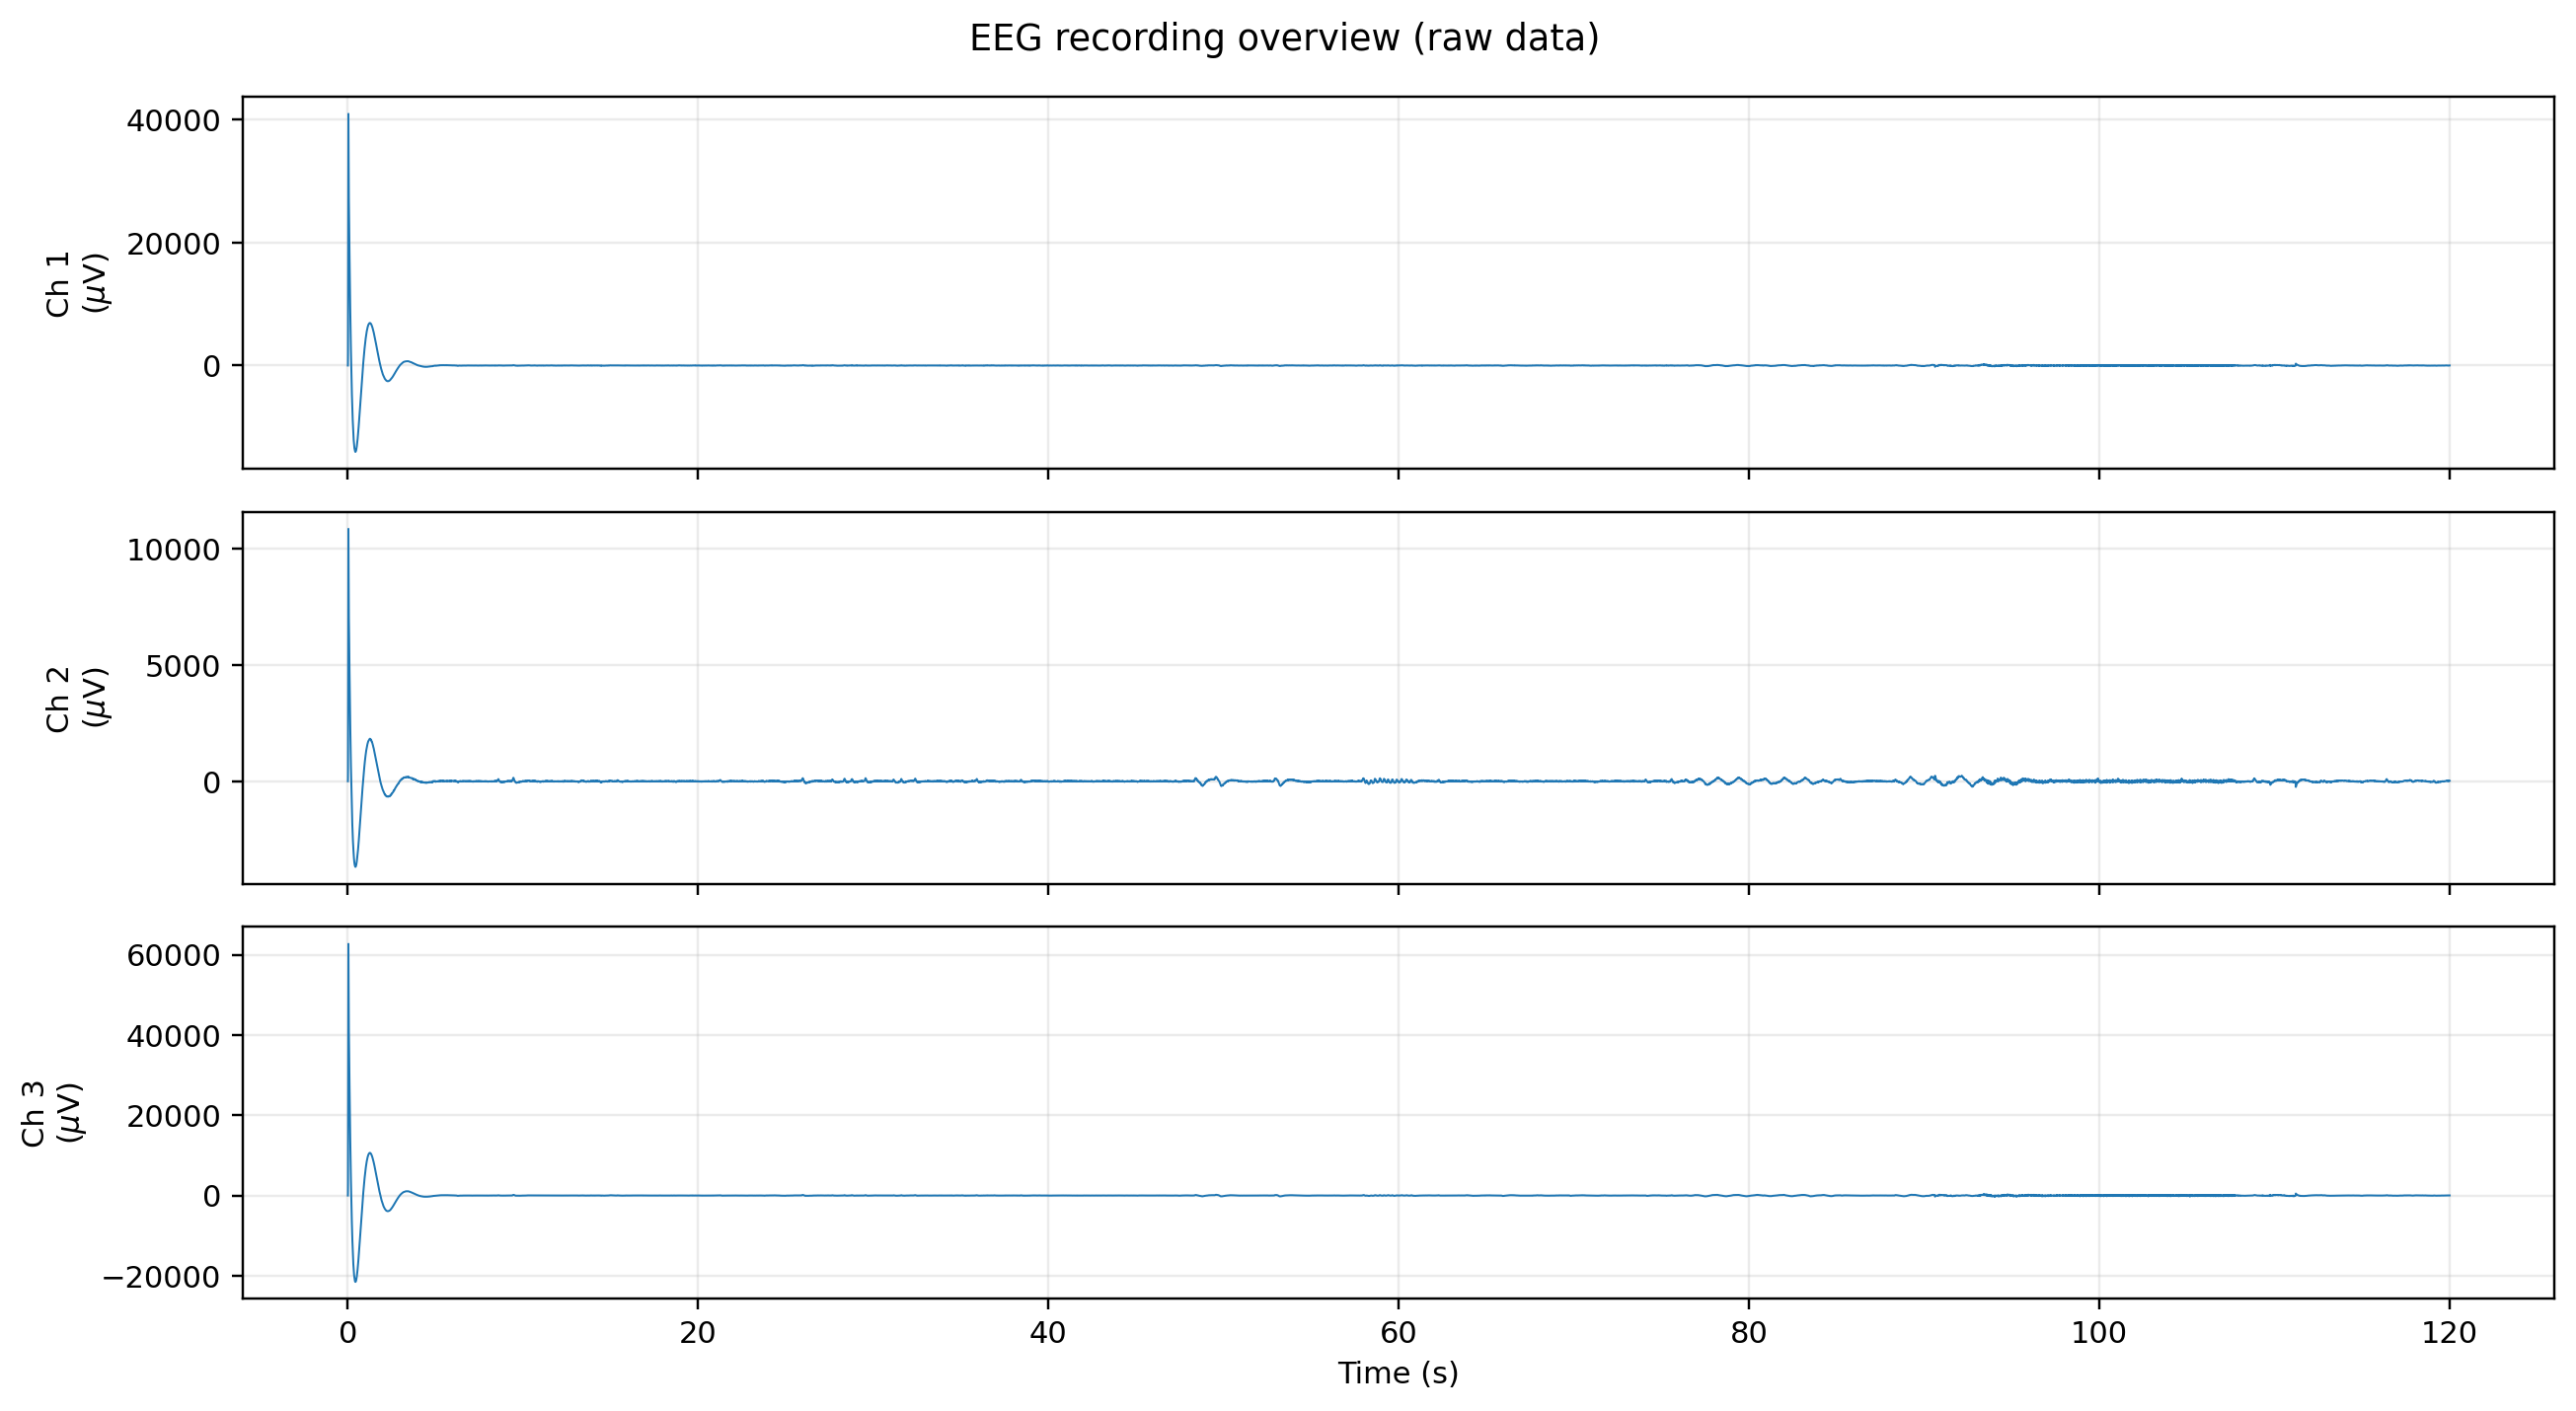
\includegraphics[width=0.98\textwidth]{eeg_recording_overview.png}
    \caption{Full-recording overview of the three columns stored in the HDF5 sample matrix. The generic labels reflect that the file does not identify the third column's physical signal type or provide anatomical electrode names.}
    \label{fig:recording_overview}
\end{figure}

\subsection{Candidate High-Amplitude Event}
Eye movements and eyelid closure can generate electro-oculographic (EOG) artifacts in frontal EEG recordings. The cornea-retina system behaves approximately as an electrical dipole, and movement of the eye changes the potential distribution measured at nearby electrodes. Blinks often produce slow, relatively high-amplitude transients, but a waveform's appearance alone is not enough to confirm that an event was an instructed blink.

\begin{figure}[H]
    \centering
    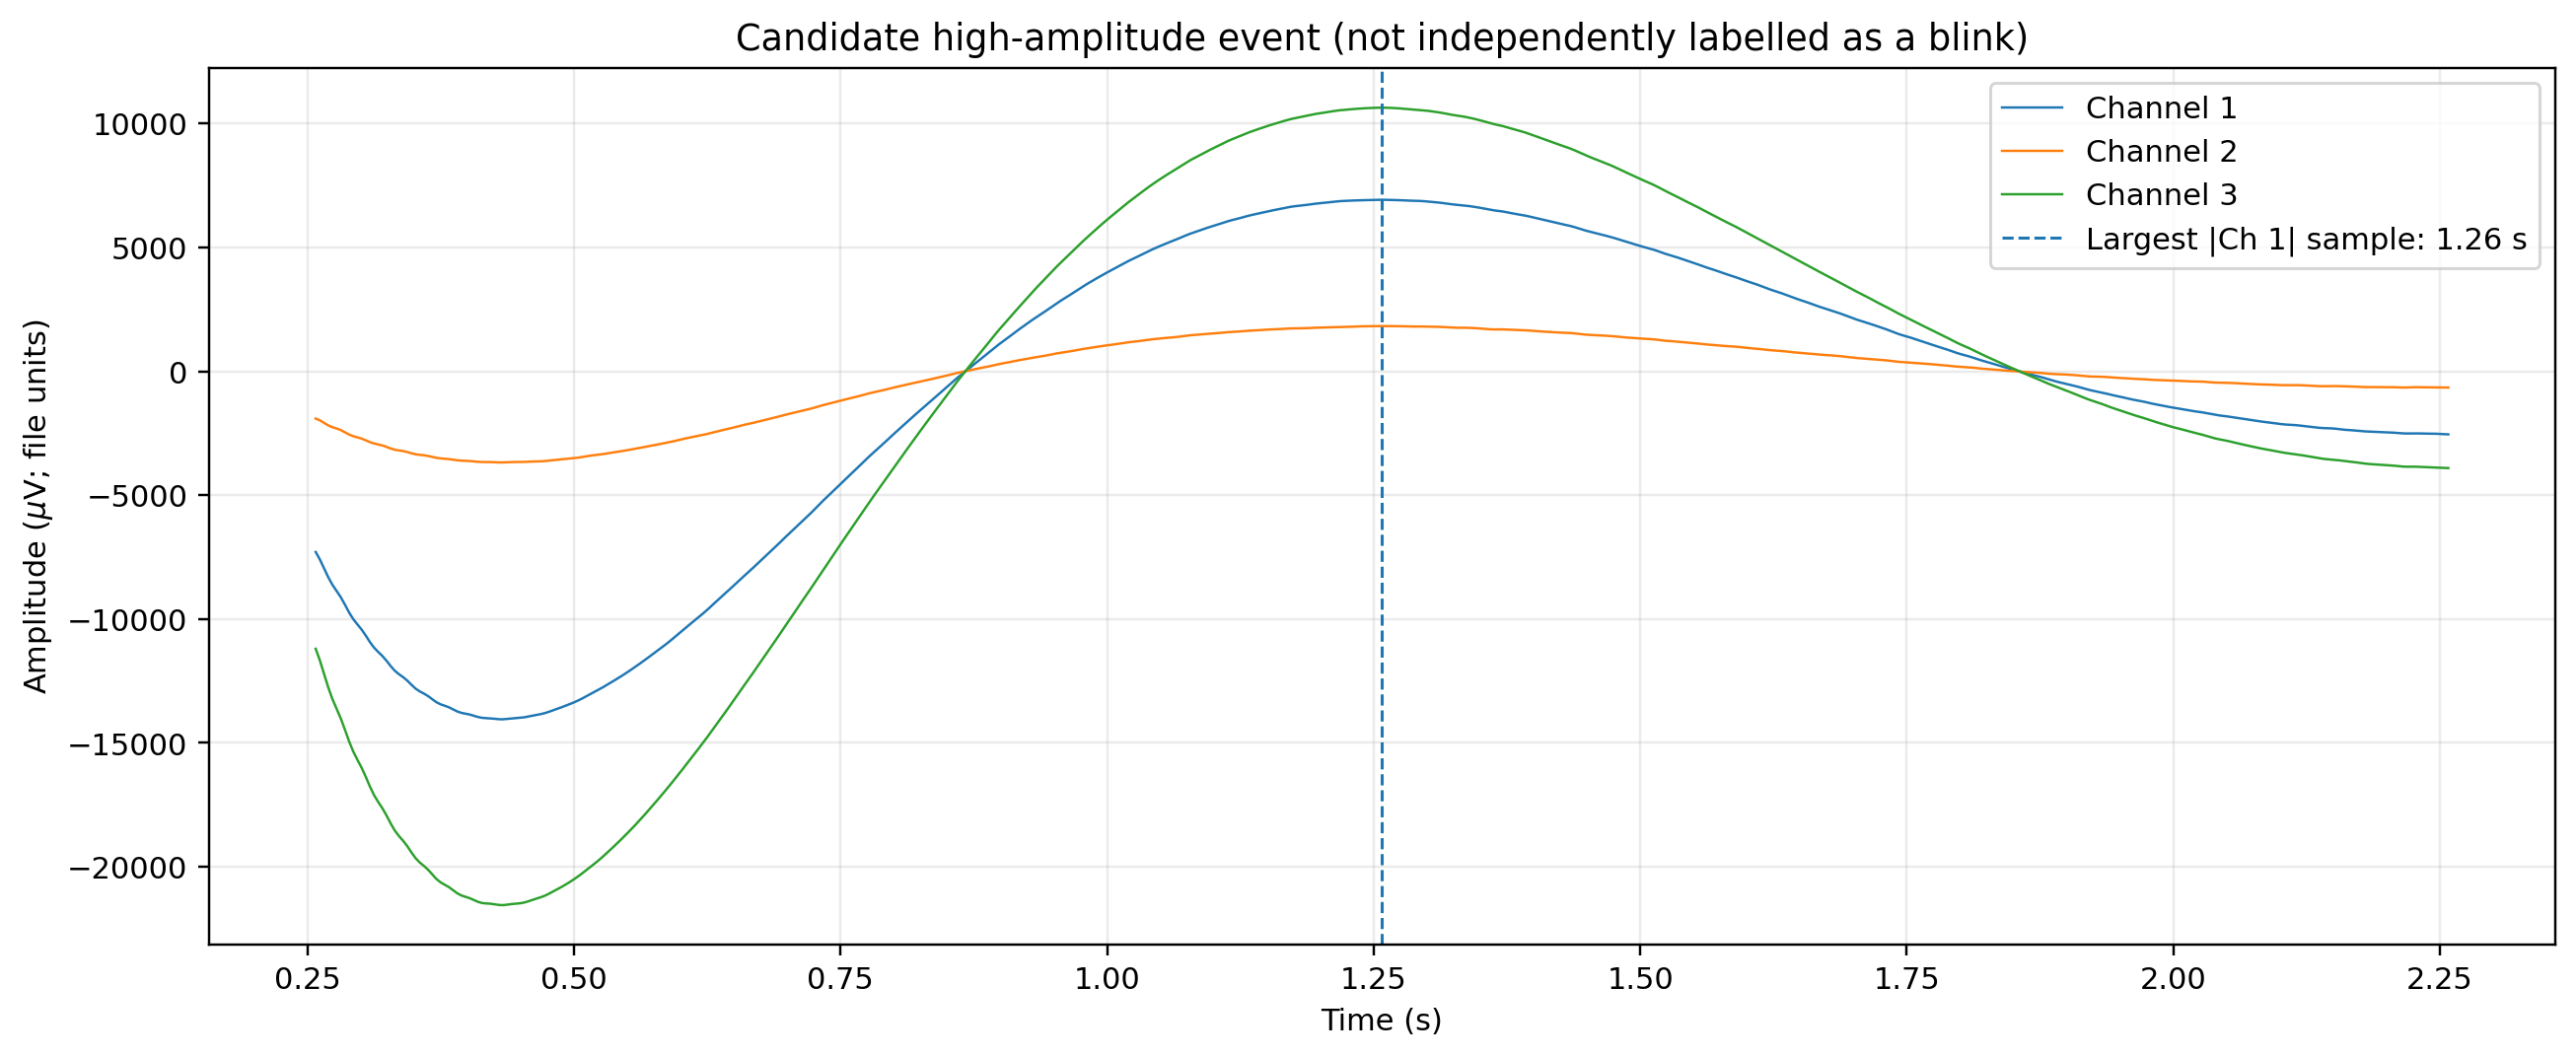
\includegraphics[width=0.98\textwidth]{eeg_blink_artifact.png}
    \caption{Two-second window around an automatically selected high-amplitude candidate event after excluding the first five seconds. The event is not independently labelled in the recording, so it should not be treated as a confirmed eye blink.}
    \label{fig:eeg_blink}
\end{figure}

The candidate was selected algorithmically from the stored samples. The recording does not include event annotations or a synchronized video/EOG channel that would independently verify the event's cause. In addition, the early part of the file contains extreme values relative to typical EEG amplitudes. This may indicate an acquisition transient, scaling or export issue, electrode artifact, or another non-neural event. The signal and acquisition settings should be verified before assigning physiological meaning to its amplitude or timing.

\subsection{Filter Comparison and Power Spectrum}
Figure~\ref{fig:eeg_notch_filtering} compares the recorded waveforms with an offline-filtered version of the signals around the selected candidate event. The offline processing applies a $50\,\mathrm{Hz}$ notch followed by a $0.5$--$8\,\mathrm{Hz}$ bandpass. The latter deliberately attenuates frequencies outside the selected low-frequency range, so changes in waveform shape should not be interpreted as evidence that ocular artifacts have been removed.

\begin{figure}[H]
    \centering
    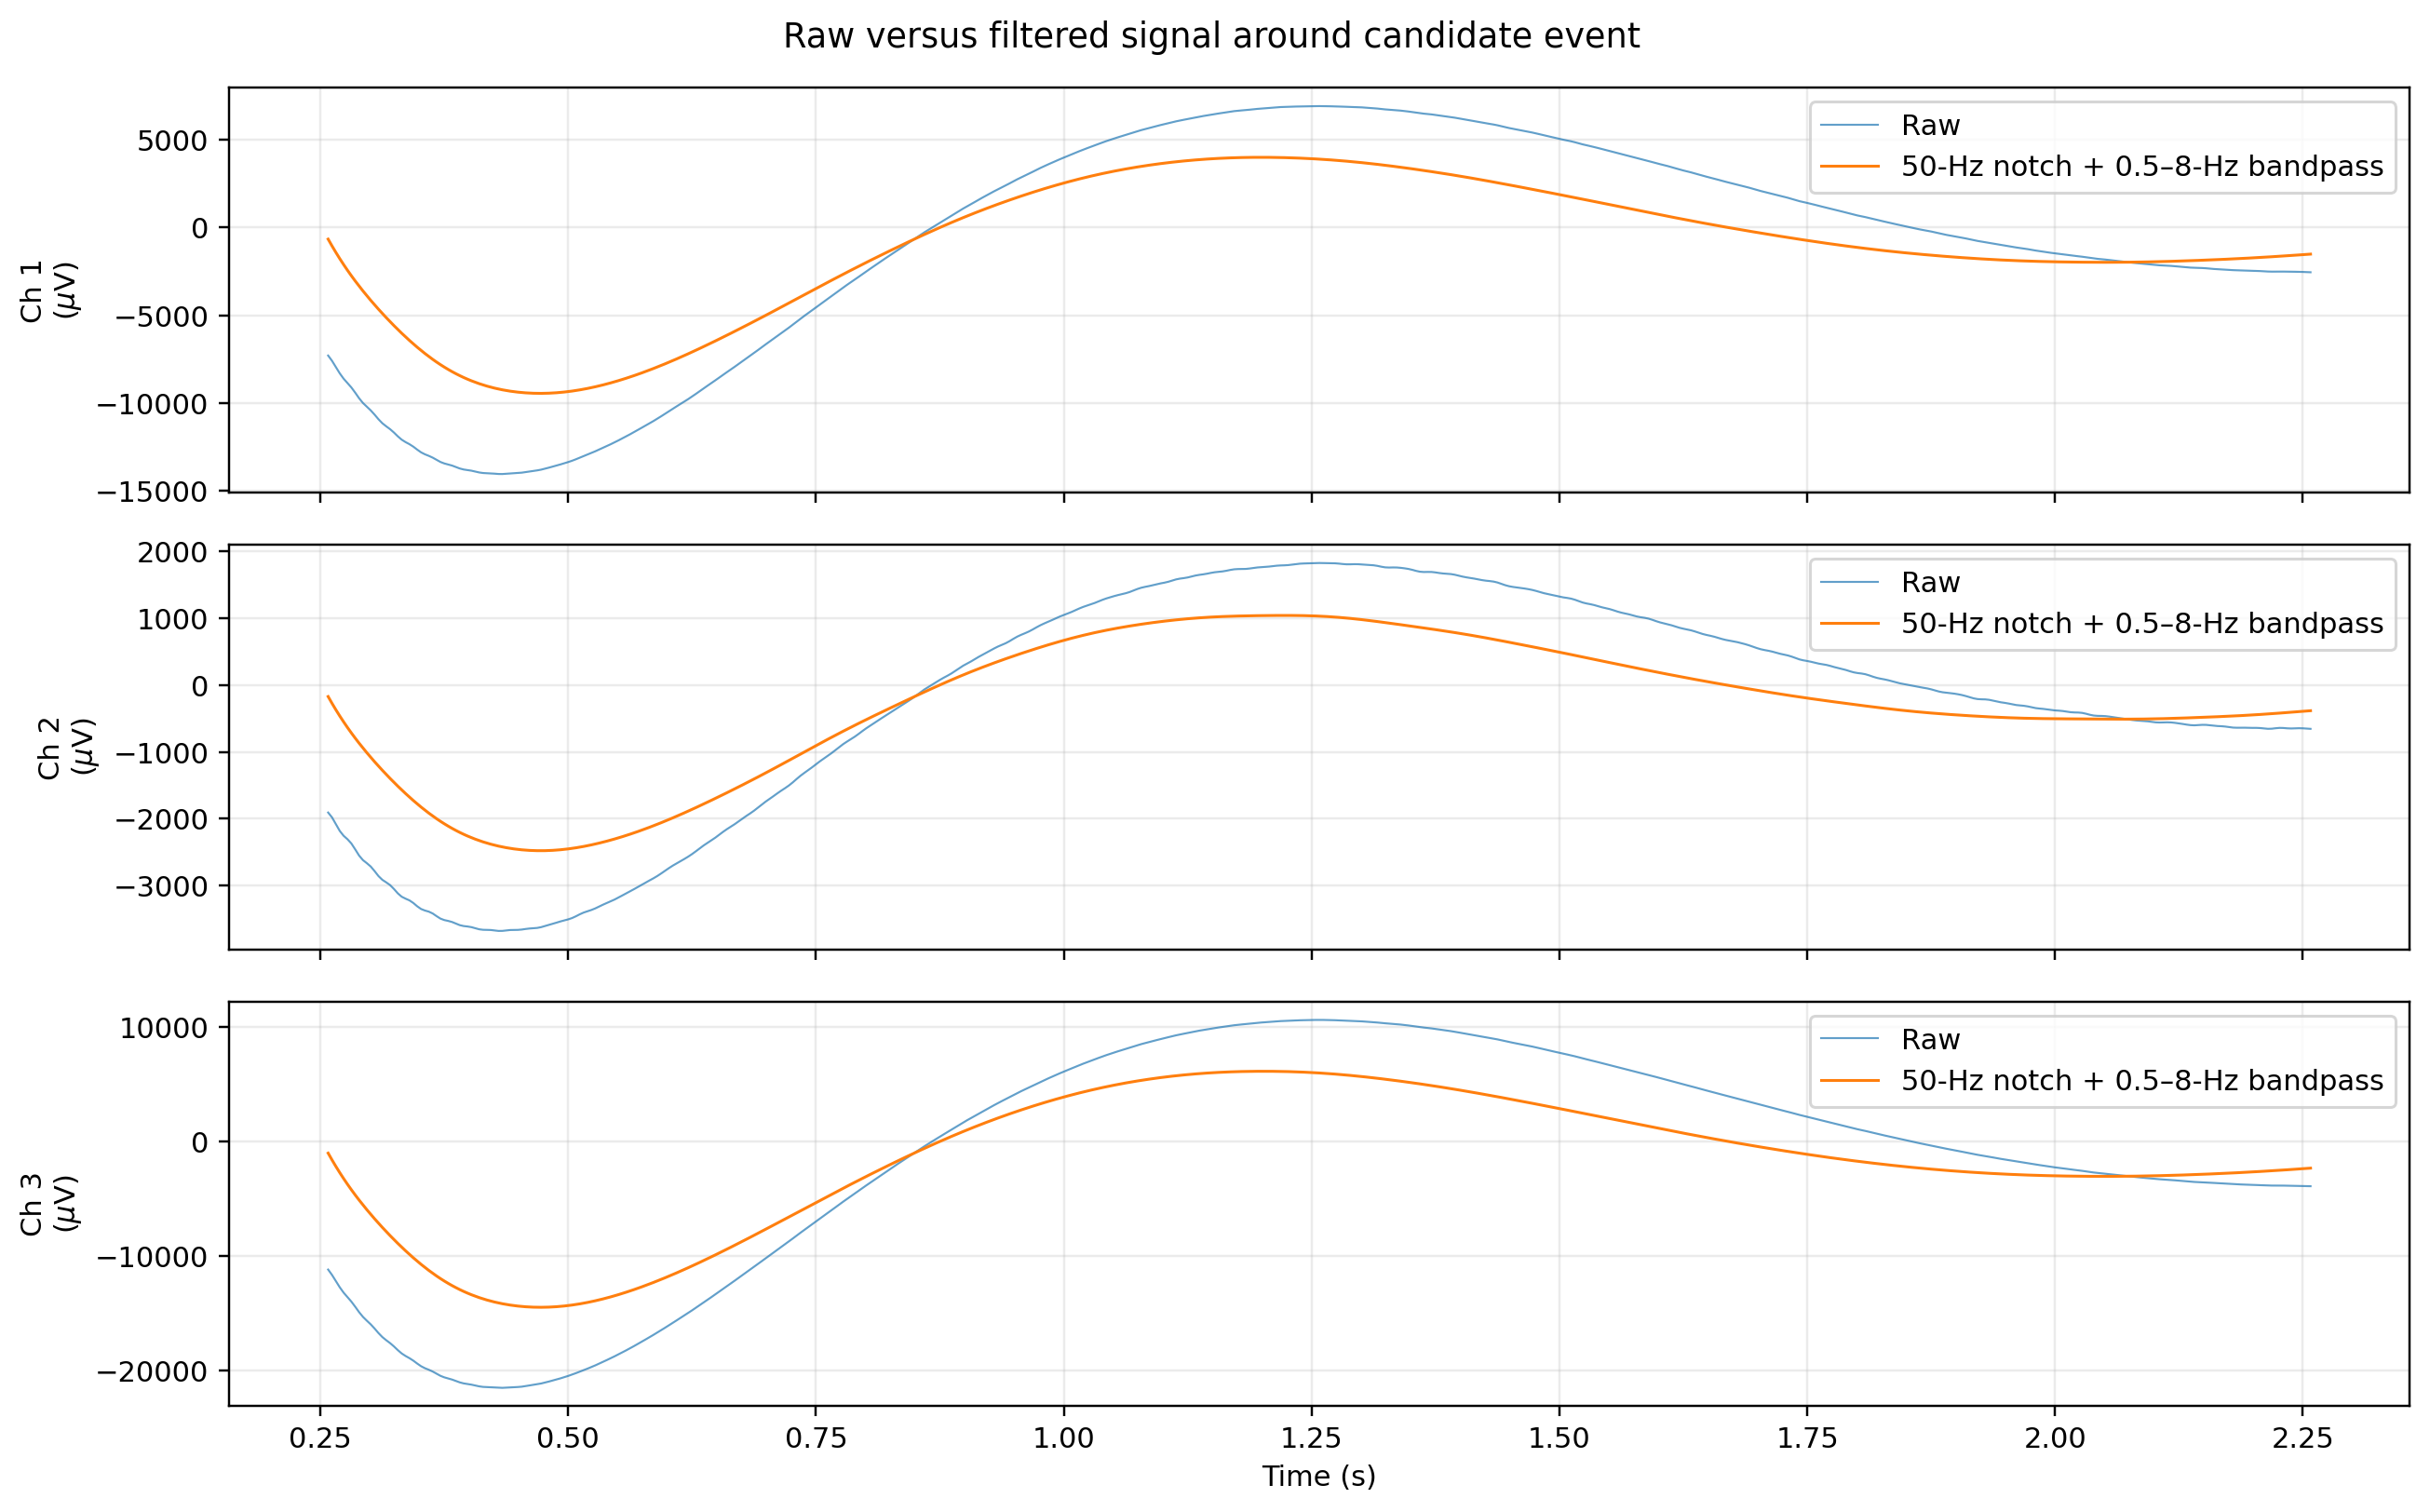
\includegraphics[width=0.98\textwidth]{eeg_notch_filtering.png}
    \caption{Raw signals and offline-filtered signals around the candidate event. The filtered trace uses a $50\,\mathrm{Hz}$ notch and a $0.5$--$8\,\mathrm{Hz}$ Butterworth bandpass.}
    \label{fig:eeg_notch_filtering}
\end{figure}

A notch filter can attenuate narrow-band mains interference when such interference is present, but it is not a general ocular-artifact-removal method. Eye-blink artifacts overlap the low-frequency range containing genuine EEG activity; simply rejecting those frequencies would also discard physiological signal. The power spectral density plot in Figure~\ref{fig:power_spectrum} provides a frequency-domain view of the recorded and filtered data.

\begin{figure}[H]
    \centering
    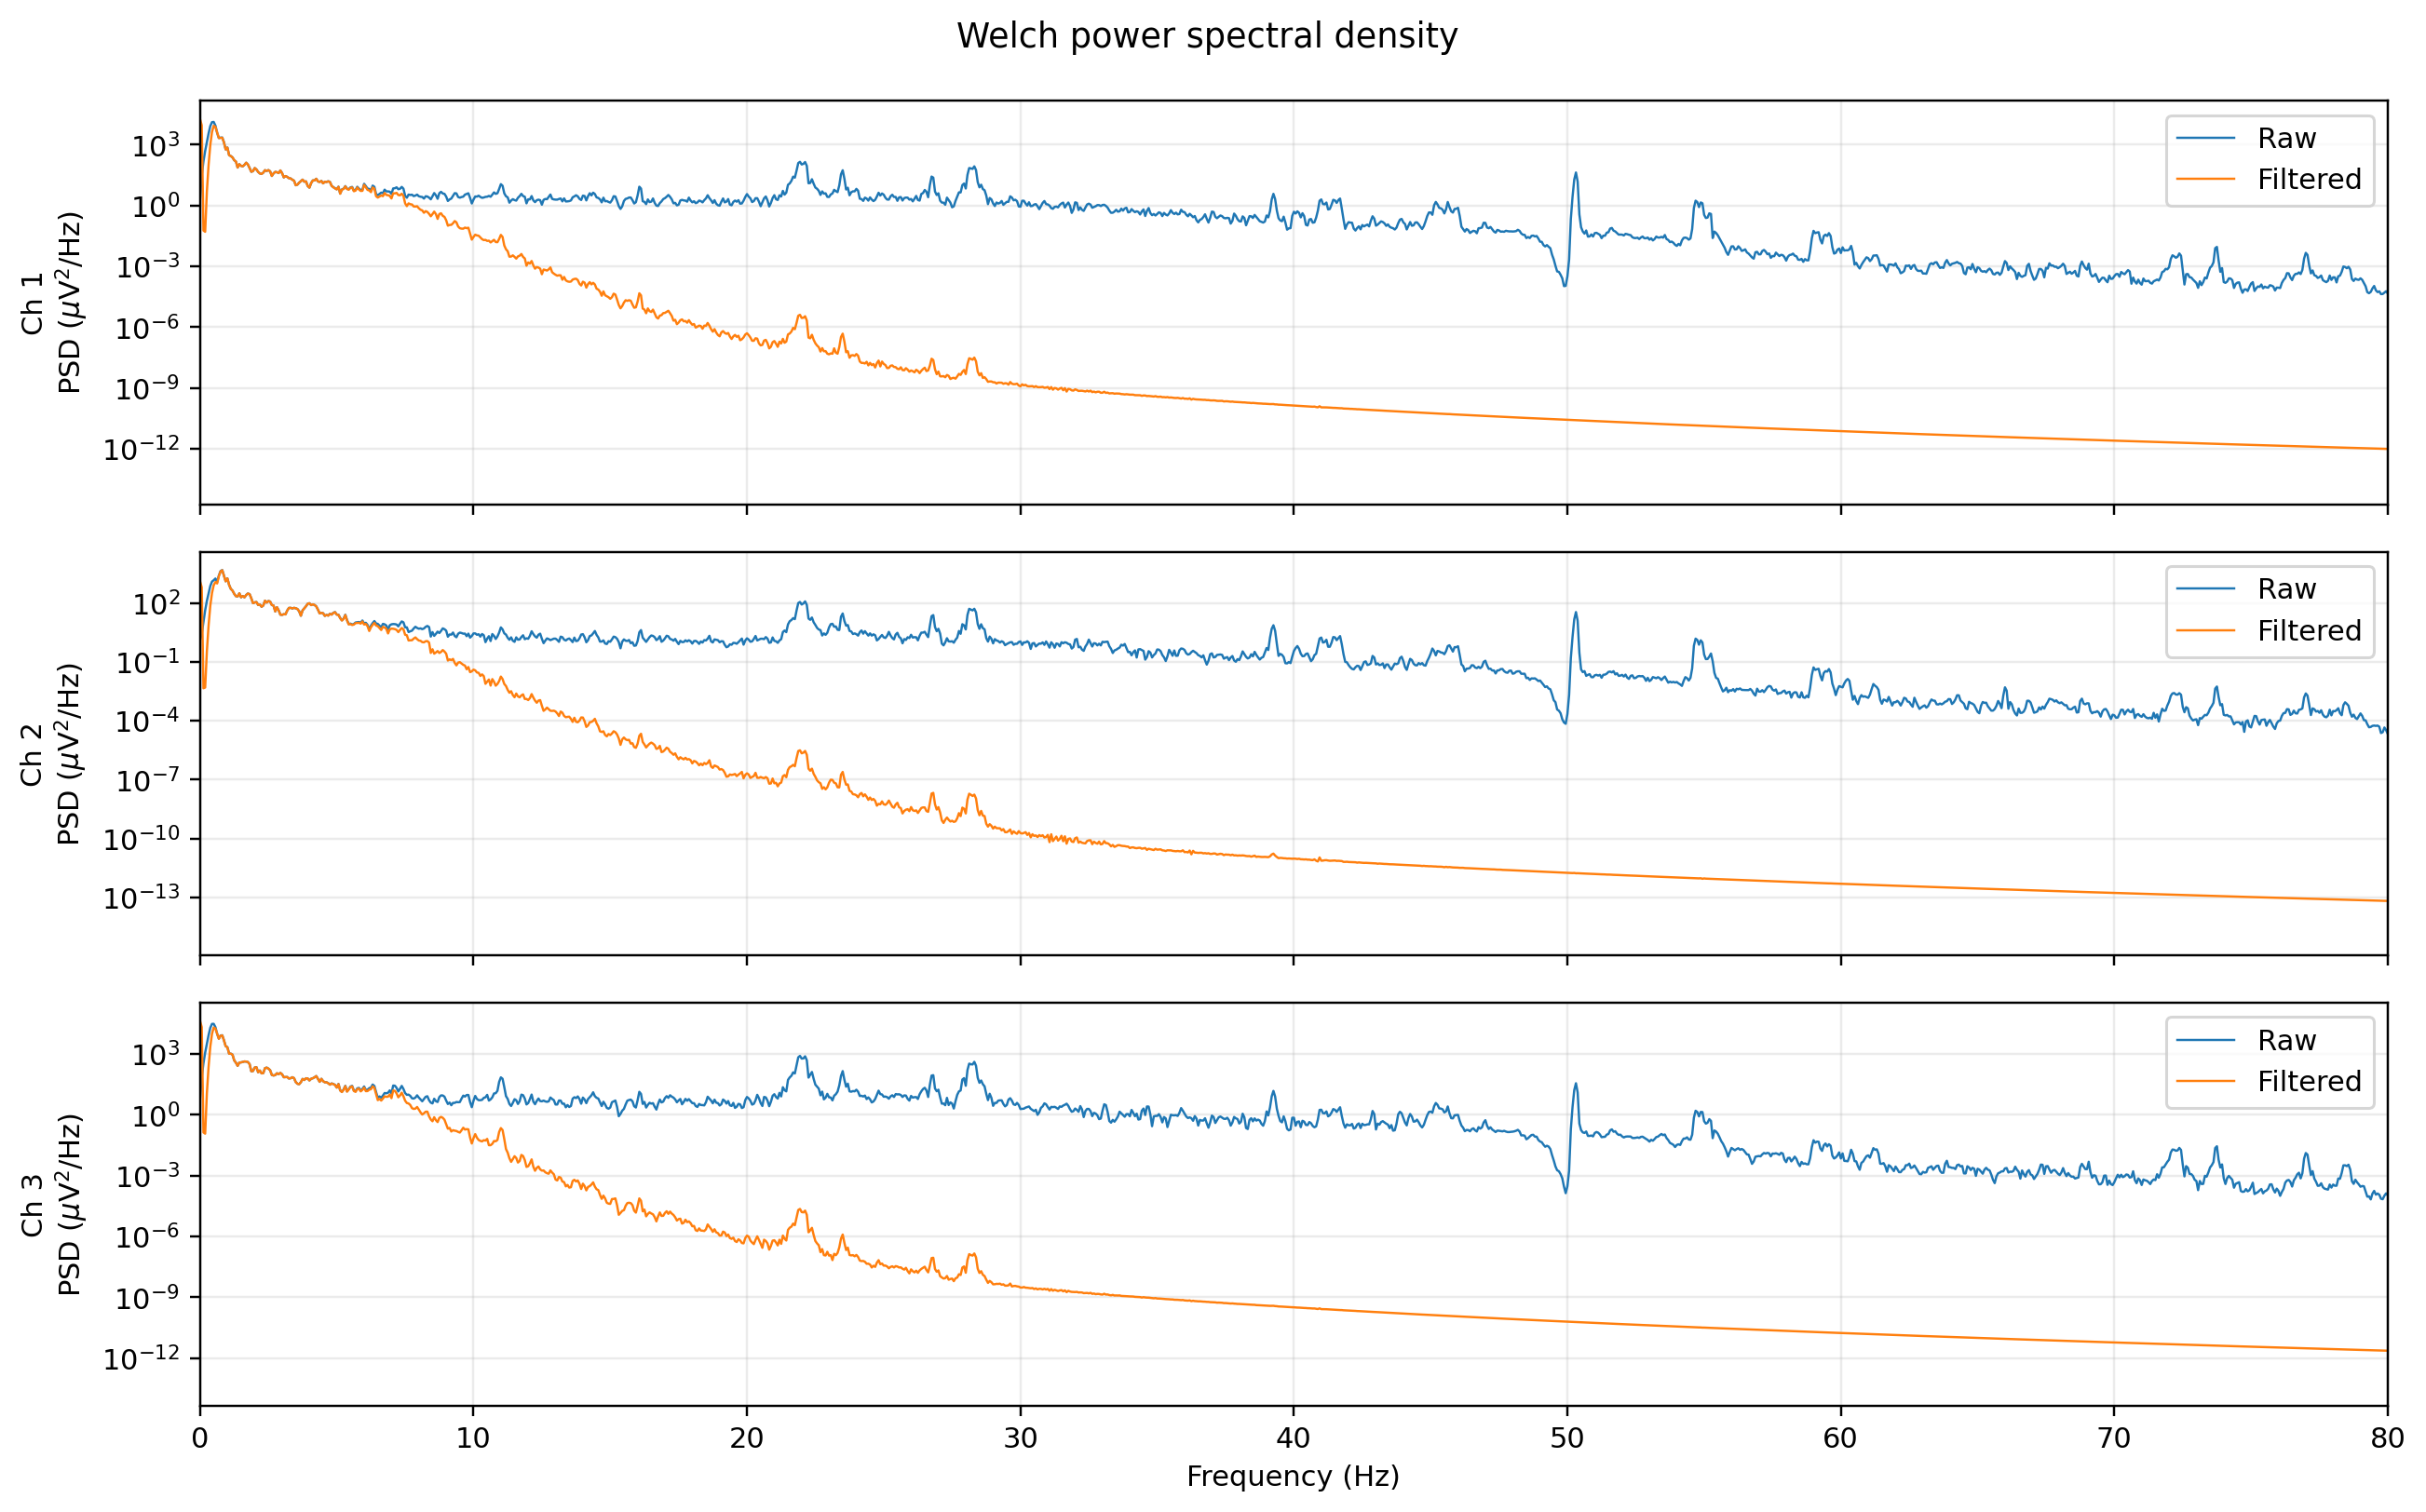
\includegraphics[width=0.98\textwidth]{eeg_power_spectrum.png}
    \caption{Welch power spectral density estimates for the raw and offline-filtered sample columns.}
    \label{fig:power_spectrum}
\end{figure}

\section{Discussion}

\subsection{Reference Electrode Principles}
The recording montage is an essential part of EEG interpretation because EEG voltages are differential measurements rather than absolute potentials. A reference that contains physiological activity or interference contributes that activity, with opposite sign, to each recorded channel. Reference selection should therefore be documented alongside channel locations and acquisition settings. Neither an ear-lobe nor a thumb electrode is guaranteed to be electrically inactive, and a comparison should be based on recordings made under well-documented, comparable conditions.

The amplifier's common-mode rejection ratio (CMRR) describes its ability to reject voltage common to both differential inputs. In simplified form, finite CMRR leaves a residual common-mode contribution at the output. Unequal electrode impedances can reduce practical rejection in real systems, but the supplied HDF5 file contains no impedance measurements or montage labels from which to quantify this effect for the present session.

\subsection{Ocular Artifacts and Filtering}
The corneo-retinal potential difference and movement of the eye can create EOG contamination at nearby scalp electrodes. Since ocular artifacts often overlap the low-frequency EEG spectrum, ordinary notch or bandpass filtering cannot reliably distinguish eye movement from brain activity based on frequency alone. In research settings, artifact handling may use additional EOG channels, careful event annotation, independent component analysis (ICA), regression, or other validated methods appropriate to the number and quality of available channels.

ICA models multichannel observations as mixtures of latent sources:
\begin{equation}
    \mathbf{x}(t)=\mathbf{A}\mathbf{s}(t),
    \label{eq:ica}
\end{equation}
where $\mathbf{x}(t)$ is the vector of measured channels, $\mathbf{A}$ is a mixing matrix, and $\mathbf{s}(t)$ is a vector of source components. Applying ICA responsibly requires an adequate number of channels, suitable data quality, and independent inspection of the components. The present recording contains three sample columns, but the metadata does not identify all channel types; therefore, successful separation of ocular and neural sources should not be assumed from this file alone.

\subsection{Data Quality and Limitations}
The main limitation is that the file metadata does not identify the exact electrode montage, anatomical channel locations, or behavioral event times. Also, the stored waveforms contain extreme early excursions that are far larger than typical scalp EEG values. These should be investigated by checking the acquisition application's displayed units, channel calibration/sensitivity settings, electrode contact, and whether the first seconds contain a startup or connection transient. Until those checks are made, peak amplitudes should not be used as physiological measurements and the selected candidate event should not be labelled as a confirmed blink.

The graphs support an exploratory review of the file's time-domain and frequency-domain structure. They do not establish an ear-lobe-versus-thumb performance result, a confirmed eye-blink amplitude, or a clinical finding.

\section{Conclusion}
The supplied HDF5 recording was inspected and plotted using a reproducible Python workflow. The file contains $30{,}725$ sample rows and three data columns recorded at $256\,\mathrm{Hz}$, corresponding to approximately $120.02\,\mathrm{s}$. Metadata identifies the acquisition device as a Guger Technologies g.HIamp system and states the recording units as microvolts.

Four plots were generated: a full-recording overview, a zoomed view of an automatically selected high-amplitude candidate event, a raw-versus-filtered comparison, and a Welch power spectral density estimate. Because the file does not label the reference montage or event markers, the analysis cannot confirm that the selected event is an eye blink or directly compare ear-lobe and thumb references. Furthermore, extreme values—particularly near the start of the recording—require validation of the signal scaling and acquisition quality before quantitative physiological interpretation.

For a defensible final report, the acquisition settings and channel labels should be checked against the recording software and laboratory worksheet. A montage comparison should use separately annotated recordings acquired under the two reference configurations.

\end{document}
